\documentclass{beamer}
\usepackage{graphicx}
\usepackage{verbatim}
\usepackage{url}
%Information to be included in the title page:
\title{Haskell or How I Learned to Stop Worrying and Love in General: Haskell for Flow Cytometry}
\author{Noah Thomas Jones}
\institute{University of Florida}
\date{}

\begin{document}

\frame{\titlepage}

\begin{frame}
  \frametitle{What is Flow?}
  \begin{figure}
    \centering
    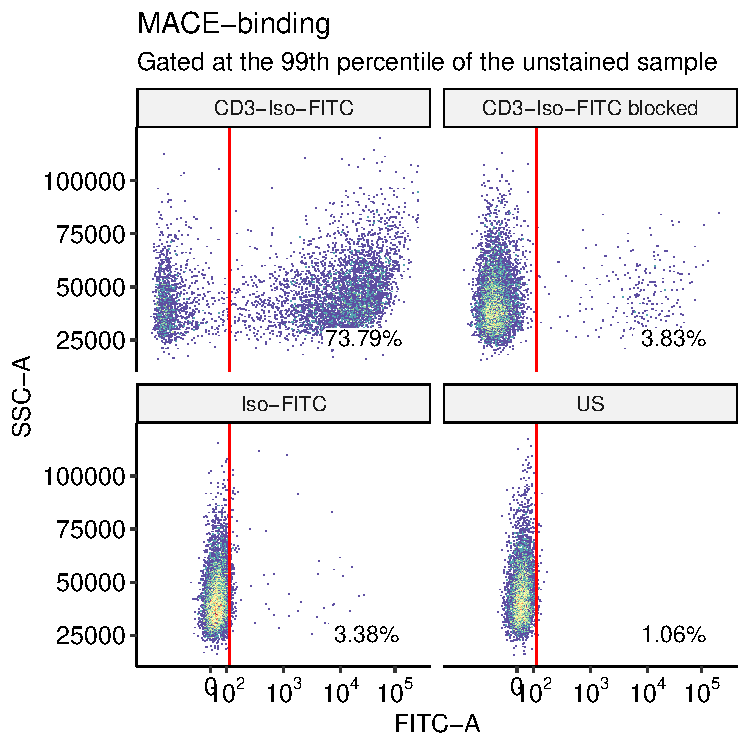
\includegraphics[width=0.45\textwidth]{./images/NJ030_MACE-binding.pdf}
    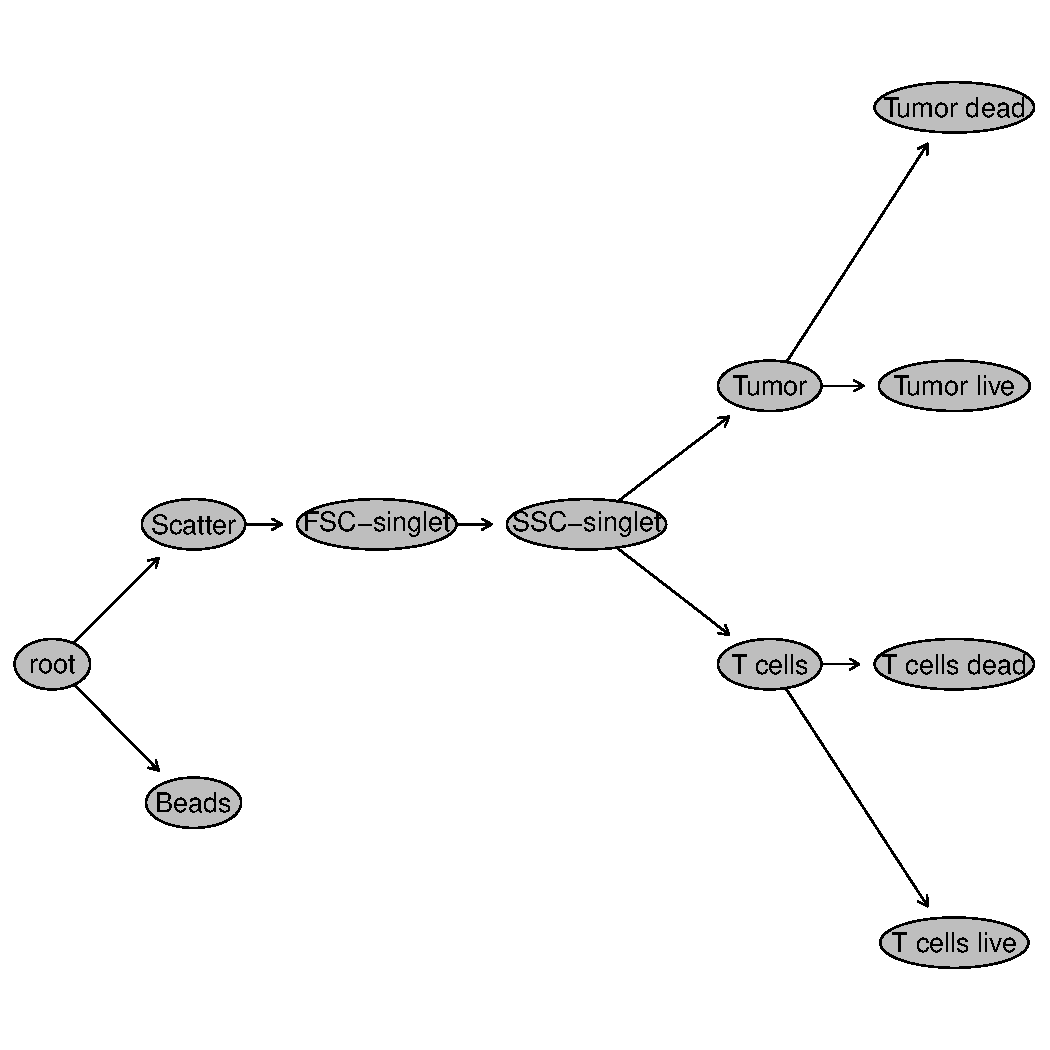
\includegraphics[width=0.45\textwidth]{./images/NJ017_gates.pdf}
    \caption{Unrelated examples: gates on fluorescent channels and
      example gating scheme.}
  \end{figure}
\end{frame}

\begin{frame}
  \frametitle{Problem Statement}
  We need flow cytometry gating scheme that does not
\end{frame}

\begin{frame}[fragile]
  \frametitle{Existing Solutions} We have a gating ML
  standard\cite{spidlen2015isac}, which does something for portability
  of gates, but of the tools used, one notable example is the R
  library \ttext{flowCore}, which after defining a \ttext{gatingset} object,
  which is an object tenuously linked to a \ttext{flowset} object, is
  modified through imperative side-effects.
\begin{verbatim}
rg1 <- rectangleGate("FSC-A"=c(50000, Inf), filterId="NonDebris")
gs_pop_add(gs, rg1, parent = "root")
## [1] 2
gs_get_pop_paths(gs)
## [1] "root" "/NonDebris"
# gate the data
recompute(gs)
## done!
\end{verbatim}
\end{frame}

\begin{frame}[fragile]
  \frametitle{Getting Started} The first objective was to write a file
  parser so that we can pull data out of our files. We can start based
  on our file specification\cite{spidlen2021data} example:
\begin{verbatim}
FCS3.0         256    1545    1792  202456       0       0 
\end{verbatim}
\end{frame}

\begin{frame}[fragile]
  \frametitle{Example}
  This function does a thing, and here we compare it to alternative package that uses GatingML
\begin{verbatim}
A proper implementation of GatingML
    \end{verbatim}
\end{frame}


\nocite{*}

\bibliography{bibliography}

\end{document}
